\section{Расчёт свойств потока}

В отличии от функций расчета PVT (физико-химических свойств флюидов) функции расчета свойства потока учитывают дополнительные параметры потока флюидов - $Q$ - дебит, объемный расход флюидов, $f_w$ - обводненность, $R_p$ - газовый фактор. В функциях свойств потока используется префикc \mintinline{vb.net}{feed_}.

Параметры потока, такие как расход ГЖС, доля газа в потоке, вязкость ГЖС важны для расчёта и анализа работы скважин и скважинного оборудования.


\subsection{feed\_q\_mix\_rc\_m3day – расход газожидкостной смеси}

Функция позволяет рассчитать объёмный расход газожидкостной смеси при заданных термобарических условиях. Объёмный расход ГЖС важен например для подбора УЭЦН в скважине, так как именно определяет в какой точке характеристики УЭЦН будет работать. При наличии свободного газа в потоке расход ГЖС может быть значительно больше расхода жидкости на поверхности фиксируемого расходомером.
$$Q_{mix,rc} = Q_{w,sc} B_w(P,T) + Q_{o,sc} B_o(P,T)  + Q_{o,sc}  (R_p - R_s(P,T)) B_g(P,T) $$

Расход ГЖС определяется как сумма расходов отдельных фаз, приведённых к соответствующим термобарическим условиям, с учётом того, что часть газа будет растворена в нефти.

\putlisting{listings/feed_q_mix_rc_m3day.lst}

\subsection{feed\_rho\_mix\_kgm3 – плотность газожидкостной смеси}

Функция позволяет рассчитать плотность газожидкостной смеси при заданных термобарических условиях. 
$$\rho_{mix,rc} = \left( \frac{\rho_{w,sc}}{B_w} f_w + \frac{\rho_{o,sc} +r_s \rho_{g,sc} }{B_o}(1-f_w) \right) (1-f_g) + \frac{ \rho_{g,sc} }{B_g} f_g $$

\putlisting{listings/feed_rho_mix_kgm3.lst}

\subsection{feed\_gas\_fraction\_d – доля газа в потоке}

Функция расчёта доли свободного газа в потоке (без учёта проскальзывания) в зависимости от термобарических условий для заданного флюида. 
$$f_g = \frac{Q_{gas\_rc} (1-k_{sep\_add})}{Q_{wat\_rc}+Q_{oil\_rc}+Q_{gas\_rc}(1-k_{sep\_add})} $$
где все объёмные расходы фаз приведены в соответствующих термобарических условиях, а $k_{sep,add}$ - дополнительный коэффициент сепарации, учитывающий удаление части свободного газа из потока.

Доля газа в потоке является одним из ключевых параметров ограничивающих производительность систем механизированной добычи - ЭЦН и других насосов.

\putlisting{listings/feed_gas_fraction_d.lst}

\subsection{feed\_p\_gas\_fraction\_atma – целевое давления для заданной доли газа в потоке}
Функция расчёта давления при котором достигается заданная доля свободного газа в потоке (без учёта проскальзывания). 
Значение давления при котором достигается определённая доля газа в потоке может быть найдено из решения уравнения, определяющего долю газа. 
$$f_g = \frac{Q_{gas\_rc} (1-k_{sep\_add})}{Q_{wat\_rc}+Q_{oil\_rc}+Q_{gas\_rc}(1-k_{sep\_add})} $$
Решение в \unf{} реализовано итеративное, методом деления отрезка пополам (дихотомия). При вызове функции пересчитывается состояние смеси с различными термобарическими условиями. Поэтому расчёт проводится относительно медленно. 

Задание $k_{sep\_add}$ позволит оценить целевое давление на приеме для ЭЦН при известной доли газа и известном ожидаемом значении сепарации газа. Отметим, что значение сепарации может быть оценено по корреляционным зависимостям. Но такие зависимости требуют знания давления сепарации, а следовательно их учет совместно с алгоритмом расчета давления при котором достигается определенная доля газа потребует итеративного решения, что выходит за рамки данной функции (например из за того, что это потребует задания дополнительных параметров конфигурации скважины).

\putlisting{listings/feed_p_gas_fraction_atma.lst}



\subsection{feed\_rp\_gas\_fraction\_m3m3 – целевой газовый фактор для заданной доли газа в потоке}
Функция расчёта газового фактора $R_p$ при котором достигается заданная доля свободного газа в потоке (без учёта проскальзывания) . 
Значение давления при котором достигается определённая доля газа в потоке может быть найдено из решения уравнения, определяющего долю газа. 
$$f_g = \frac{Q_{gas\_rc} (1-k_{sep\_add})}{Q_{wat\_rc}+Q_{oil\_rc}+Q_{gas\_rc}(1-k_{sep\_add})} $$

Решение в \unf{} реализовано с использованием итераций, методом деления отрезка пополам (дихотомия). При вызове функции  состояние смеси пересчитывается с различными термобарическими условиями. Поэтому расчёт проводится относительно медленно. 

Задание $k_{sep\_add}$ позволит оценить целевой газовый фактор при известной доли газа, давлении на приеме и ожидаемом значении сепарации газа. Отметим, что значение сепарации может быть оценено по корреляционным зависимостям. Но такие зависимости требуют знания как давления сепарации так и газового фактора, а следовательно их учет совместно с алгоритмом расчета газового фактора при котором достигается определенная доля газа потребует итеративного решения, что выходит за рамки данной функции (например из за того, что это потребует задания дополнительных параметров конфигурации скважины).

\putlisting{listings/feed_rp_gas_fraction_m3m3.lst}

\section{Сепарация газа в скважине}
В скважинах оборудованных системами механизированной добычи нефти важную роль играет процесс сепарации газа на приёме насоса. Под сепарацией газа понимается отделение части свободного газа из потока и перенаправление его по отдельному гидравлическому каналу на поверхность. В результате сепарации газа меняются свойства флюида, поступающего в насос и НКТ выше насоса. В частности меняются давление насыщения и газосодержание при давлении насыщения для флюида после сепарации. Более детальные модели флюида и сепарации могут показать, что при сепарации может поменяться и другие параметры - например состав газа после разгазирования. В модели нелетучей нефти реализованной в \unf{} эти эффекты не учитываются.


\begin{figure}[H]
	\centering
		

\tikzset{every picture/.style={line width=0.75pt}} %set default line width to 0.75pt        

\begin{tikzpicture}[x=0.75pt,y=0.75pt,yscale=-1,xscale=1]
%uncomment if require: \path (0,406); %set diagram left start at 0, and has height of 406

%Shape: Rectangle [id:dp04480742808021354] 
\draw  [fill={rgb, 255:red, 155; green, 155; blue, 155 }  ,fill opacity=1 ] (312,64.14) -- (351.5,64.14) -- (351.5,114.5) -- (312,114.5) -- cycle ;
%Shape: Rectangle [id:dp3210354209072095] 
\draw  [line width=2.25]  (259.42,64.14) -- (404.08,64.14) -- (404.08,352) -- (259.42,352) -- cycle ;
%Shape: Rectangle [id:dp11917689807401133] 
\draw  [fill={rgb, 255:red, 155; green, 155; blue, 155 }  ,fill opacity=1 ] (296.75,114.5) -- (366.75,114.5) -- (366.75,314.5) -- (296.75,314.5) -- cycle ;
%Shape: Rectangle [id:dp22447305445205257] 
\draw  [fill={rgb, 255:red, 255; green, 255; blue, 255 }  ,fill opacity=1 ] (305.89,238.94) -- (310.33,238.94) -- (310.33,269.56) -- (305.89,269.56) -- cycle ;
%Shape: Rectangle [id:dp05751039520762724] 
\draw  [fill={rgb, 255:red, 255; green, 255; blue, 255 }  ,fill opacity=1 ] (314.33,238.94) -- (318.78,238.94) -- (318.78,269.56) -- (314.33,269.56) -- cycle ;
%Shape: Rectangle [id:dp6083474962263296] 
\draw  [fill={rgb, 255:red, 255; green, 255; blue, 255 }  ,fill opacity=1 ] (322.11,238.94) -- (326.56,238.94) -- (326.56,269.56) -- (322.11,269.56) -- cycle ;
%Shape: Rectangle [id:dp9699991258462393] 
\draw  [fill={rgb, 255:red, 255; green, 255; blue, 255 }  ,fill opacity=1 ] (329.53,238.94) -- (333.97,238.94) -- (333.97,269.56) -- (329.53,269.56) -- cycle ;
%Shape: Rectangle [id:dp5276274421172025] 
\draw  [fill={rgb, 255:red, 255; green, 255; blue, 255 }  ,fill opacity=1 ] (337,238.94) -- (341.44,238.94) -- (341.44,269.56) -- (337,269.56) -- cycle ;
%Shape: Rectangle [id:dp8686039431642814] 
\draw  [fill={rgb, 255:red, 255; green, 255; blue, 255 }  ,fill opacity=1 ] (344.78,238.94) -- (349.22,238.94) -- (349.22,269.56) -- (344.78,269.56) -- cycle ;
%Shape: Rectangle [id:dp024923249699371652] 
\draw  [fill={rgb, 255:red, 255; green, 255; blue, 255 }  ,fill opacity=1 ] (352.56,238.94) -- (357,238.94) -- (357,269.56) -- (352.56,269.56) -- cycle ;
%Shape: Rectangle [id:dp24614630976896423] 
\draw  [fill={rgb, 255:red, 255; green, 255; blue, 255 }  ,fill opacity=1 ] (360.11,238.94) -- (364.56,238.94) -- (364.56,269.56) -- (360.11,269.56) -- cycle ;
%Shape: Rectangle [id:dp4580617305504924] 
\draw  [fill={rgb, 255:red, 255; green, 255; blue, 255 }  ,fill opacity=1 ] (298.78,238.94) -- (303.22,238.94) -- (303.22,269.56) -- (298.78,269.56) -- cycle ;
%Curve Lines [id:da46150758694693694] 
\draw [color={rgb, 255:red, 74; green, 144; blue, 226 }  ,draw opacity=1 ]   (282.2,352) .. controls (281.45,261.49) and (287.15,263.11) .. (299.52,257.34) ;
\draw [shift={(302.2,256)}, rotate = 511.33] [fill={rgb, 255:red, 74; green, 144; blue, 226 }  ,fill opacity=1 ][line width=0.08]  [draw opacity=0] (10.72,-5.15) -- (0,0) -- (10.72,5.15) -- (7.12,0) -- cycle    ;
%Shape: Circle [id:dp04721201185159396] 
\draw  [fill={rgb, 255:red, 255; green, 255; blue, 255 }  ,fill opacity=1 ] (304.99,174.01) .. controls (306.3,170.48) and (308.78,169.68) .. (310.52,172.22) .. controls (312.26,174.75) and (312.61,179.67) .. (311.3,183.19) .. controls (309.99,186.72) and (307.51,187.52) .. (305.77,184.98) .. controls (304.03,182.45) and (303.68,177.53) .. (304.99,174.01) -- cycle ;
%Shape: Circle [id:dp5883852152967295] 
\draw  [fill={rgb, 255:red, 255; green, 255; blue, 255 }  ,fill opacity=1 ] (350.59,174.01) .. controls (351.9,170.48) and (354.38,169.68) .. (356.12,172.22) .. controls (357.86,174.75) and (358.21,179.67) .. (356.9,183.19) .. controls (355.59,186.72) and (353.11,187.52) .. (351.37,184.98) .. controls (349.63,182.45) and (349.28,177.53) .. (350.59,174.01) -- cycle ;
%Curve Lines [id:da5619628529147929] 
\draw [color={rgb, 255:red, 74; green, 144; blue, 226 }  ,draw opacity=1 ]   (308.54,178.6) .. controls (288.8,173.65) and (285.1,176) .. (286.11,97.21) ;
\draw [shift={(286.14,94.8)}, rotate = 450.78] [fill={rgb, 255:red, 74; green, 144; blue, 226 }  ,fill opacity=1 ][line width=0.08]  [draw opacity=0] (10.72,-5.15) -- (0,0) -- (10.72,5.15) -- (7.12,0) -- cycle    ;
%Curve Lines [id:da7420889905281607] 
\draw [color={rgb, 255:red, 74; green, 144; blue, 226 }  ,draw opacity=1 ]   (269.4,352) .. controls (268.97,261.5) and (271.07,125.81) .. (271.01,97.45) ;
\draw [shift={(271,94.8)}, rotate = 449.4] [fill={rgb, 255:red, 74; green, 144; blue, 226 }  ,fill opacity=1 ][line width=0.08]  [draw opacity=0] (10.72,-5.15) -- (0,0) -- (10.72,5.15) -- (7.12,0) -- cycle    ;
%Curve Lines [id:da1955664158849284] 
\draw [color={rgb, 255:red, 74; green, 144; blue, 226 }  ,draw opacity=1 ]   (331.75,231.56) .. controls (331.45,207.23) and (331.44,241.87) .. (331.75,97) ;
\draw [shift={(331.75,94.8)}, rotate = 450.12] [fill={rgb, 255:red, 74; green, 144; blue, 226 }  ,fill opacity=1 ][line width=0.08]  [draw opacity=0] (10.72,-5.15) -- (0,0) -- (10.72,5.15) -- (7.12,0) -- cycle    ;
%Curve Lines [id:da5073323315189147] 
\draw [color={rgb, 255:red, 74; green, 144; blue, 226 }  ,draw opacity=1 ]   (331.75,230.44) .. controls (330.74,183.59) and (324.76,182.05) .. (316.18,179.48) ;
\draw [shift={(313.4,178.58)}, rotate = 379.94] [fill={rgb, 255:red, 74; green, 144; blue, 226 }  ,fill opacity=1 ][line width=0.08]  [draw opacity=0] (10.72,-5.15) -- (0,0) -- (10.72,5.15) -- (7.12,0) -- cycle    ;
%Curve Lines [id:da18312163514470803] 
\draw [color={rgb, 255:red, 74; green, 144; blue, 226 }  ,draw opacity=1 ]   (331.75,231.17) .. controls (330.77,185.6) and (339.02,182.33) .. (345.86,179.93) ;
\draw [shift={(348.56,178.89)}, rotate = 514.89] [fill={rgb, 255:red, 74; green, 144; blue, 226 }  ,fill opacity=1 ][line width=0.08]  [draw opacity=0] (10.72,-5.15) -- (0,0) -- (10.72,5.15) -- (7.12,0) -- cycle    ;
%Curve Lines [id:da5609474333970248] 
\draw [color={rgb, 255:red, 74; green, 144; blue, 226 }  ,draw opacity=1 ]   (353.74,178.6) .. controls (374.5,175.74) and (380.34,176.04) .. (381.54,97.21) ;
\draw [shift={(381.57,94.8)}, rotate = 450.78] [fill={rgb, 255:red, 74; green, 144; blue, 226 }  ,fill opacity=1 ][line width=0.08]  [draw opacity=0] (10.72,-5.15) -- (0,0) -- (10.72,5.15) -- (7.12,0) -- cycle    ;
%Curve Lines [id:da942989625089206] 
\draw [color={rgb, 255:red, 74; green, 144; blue, 226 }  ,draw opacity=1 ]   (394.29,352) .. controls (393.86,261.5) and (394.33,125.81) .. (394.16,97.45) ;
\draw [shift={(394.14,94.8)}, rotate = 449.4] [fill={rgb, 255:red, 74; green, 144; blue, 226 }  ,fill opacity=1 ][line width=0.08]  [draw opacity=0] (10.72,-5.15) -- (0,0) -- (10.72,5.15) -- (7.12,0) -- cycle    ;
%Curve Lines [id:da2534809401724647] 
\draw [color={rgb, 255:red, 74; green, 144; blue, 226 }  ,draw opacity=1 ]   (381.98,352) .. controls (381.21,259.56) and (377.98,263.5) .. (358.91,258.24) ;
\draw [shift={(356.11,257.42)}, rotate = 377.19] [fill={rgb, 255:red, 74; green, 144; blue, 226 }  ,fill opacity=1 ][line width=0.08]  [draw opacity=0] (10.72,-5.15) -- (0,0) -- (10.72,5.15) -- (7.12,0) -- cycle    ;
%Shape: Rectangle [id:dp25186132731738486] 
\draw  [color={rgb, 255:red, 255; green, 255; blue, 255 }  ,draw opacity=1 ][fill={rgb, 255:red, 255; green, 255; blue, 255 }  ,fill opacity=1 ] (249.86,58.29) -- (411.29,58.29) -- (411.29,70.29) -- (249.86,70.29) -- cycle ;
%Shape: Rectangle [id:dp3766484711992675] 
\draw  [color={rgb, 255:red, 255; green, 255; blue, 255 }  ,draw opacity=1 ][fill={rgb, 255:red, 255; green, 255; blue, 255 }  ,fill opacity=1 ] (251.43,346.29) -- (414.71,346.29) -- (414.71,358.57) -- (251.43,358.57) -- cycle ;





\end{tikzpicture}
		\caption{Схема линий тока газа на приеме ЭЦН}
		\label{ris:separation_scheme}
\end{figure}

В скважине с ЭЦН работают два механизма сепарации свободного газа из потока, схематично показанные на рисунке \ref{ris:separation_scheme} - естественная или натуральная сепарация газа, когда часть свободного газа за счет сил всплытия проходит мимо приема насоса и искусственная сепарация с применением газосепаратора, когда часть свободного газа выталкивается из насоса, обычно за счет центробежных сил. 

Оценка этих механизмов, а также расчёт общей сепарации могут быть проведены приведёнными ниже функциями.

\subsection{well\_ksep\_natural\_d – естественная сепарация газа}
Функция рассчитывает естественную сепарацию газа на приёме насоса в скважине с использованием корреляции Маркеса \cite{Marquez_2003} . Результат - безразмерная величина в диапазоне от 0 до 1. 

\putlisting{listings/well_ksep_natural_d.lst}

%\subsection{ESP\_ksep\_gasseparator\_d – сепарация газа роторным газосепаратором}
%Функция рассчитывает сепарацию газа с использованием роторного газосепаратора, являющегося обычно частью компоновки УЭЦН. Данный расчет основан на результатах испытания характеристик роторных газосепараторов, выполненных в РГУ нефти и газа имени И.М.Губкина \cite{SPE_117415_2008}. 

%Следует отметить, что несмотря на хорошее соответствие промысловых исследований и расчетов с использованием корреляции для естественной и искусственной сепарации \cite{SPE_117415_2008} к результатам стендовых исследований стоит относится с осторожностью. Основой осторожности могут быть следующие соображения: характеристики различных газосепараторов достаточно сильно отличаются друг от друга - есть удачные конструкции и не очень, при этом результаты стендовых испытаний доступны только для ограниченного набора конструкций, стендовые условия достаточно сильно отличаются от скважинных - ниже давление, другие модельные рабочие жидкости, точно оценить коэффициент сепарации газосепаратора в промысловых условиях затруднительно - набор таких данных для сравнения ограничен. 

%Тем не менее изучение результатов стендовых испытаний полезно при проведении расчетов и развивает инженерную интуицию. 

%\putlisting{listings/ESP_gassep_ksep_d.lst}


\subsection{well\_ksep\_total\_d – общая сепарация газа}

Функция рассчитывает полную сепарацию газа на приёме насосе в скважине по известным значениям естественной сепарации газа и коэффициента сепарации газосепаратора. Результат - безразмерная величина в диапазоне от 0 до 1. 

$$K_{sep\_total} = K_{sep\_nat} + (1-K_{sep\_nat}) K_{sep\_gassep}$$

\putlisting{listings/well_ksep_total_d.lst}

\section{Расчёт многофазного потока в штуцере}


Штуцер или локальное гидравлическое сопротивление - элемент скважины или системы трубопроводов, применяемых для создания дополнительного перепада давления в системе и ограничения потока. 
Возможны различные варианты реализации штуцера - со штуцерной камерой, с угловым краном, позволяющим менять диаметр штуцера и другие.
Ключевым параметром штуцера является диаметр \(d_{choke} \) определяющий его способность к ограничению потока. 

\begin{figure}[H]
	\begin{center}
	    		% https://www.mathcha.io/editor# использован для построения картинок



		
		\tikzset{every picture/.style={line width=0.75pt}} %set default line width to 0.75pt        
		
		\begin{tikzpicture}[x=0.75pt,y=0.75pt,yscale=-1,xscale=1]
		%uncomment if require: \path (0,300); %set diagram left start at 0, and has height of 300
		
		%Shape: Rectangle [id:dp8089540927658381] 
		\draw  [color={rgb, 255:red, 0; green, 0; blue, 0 }  ,draw opacity=1 ][fill={rgb, 255:red, 155; green, 155; blue, 155 }  ,fill opacity=1 ][line width=2.25]  (92,42) -- (570.83,42) -- (570.83,56.33) -- (92,56.33) -- cycle ;
		%Shape: Rectangle [id:dp7288541809010827] 
		\draw  [fill={rgb, 255:red, 155; green, 155; blue, 155 }  ,fill opacity=1 ][line width=2.25]  (92,227) -- (570.83,227) -- (570.83,241) -- (92,241) -- cycle ;
		%Shape: Rectangle [id:dp666453613189492] 
		\draw  [color={rgb, 255:red, 0; green, 0; blue, 0 }  ,draw opacity=1 ][fill={rgb, 255:red, 155; green, 155; blue, 155 }  ,fill opacity=1 ][line width=2.25]  (323.83,56.33) -- (341.17,56.33) -- (341.17,118.67) -- (323.83,118.67) -- cycle ;
		%Shape: Rectangle [id:dp015115451250117262] 
		\draw  [fill={rgb, 255:red, 155; green, 155; blue, 155 }  ,fill opacity=1 ][line width=2.25]  (323.83,165) -- (341.83,165) -- (341.83,226.83) -- (323.83,226.83) -- cycle ;
		%Right Arrow [id:dp058738740185342975] 
		\draw   (231,133.5) -- (274.56,133.5) -- (274.56,127) -- (289.83,140) -- (274.56,153) -- (274.56,146.5) -- (231,146.5) -- cycle ;
		%Straight Lines [id:da28021737295590965] 
		\draw    (341,119) -- (455,119) ;
		
		
		%Straight Lines [id:da8575303554097866] 
		\draw    (341,165) -- (455,165) ;
		
		
		%Straight Lines [id:da44299065539354565] 
		\draw    (440,120.89) -- (440,161.67) ;
		\draw [shift={(440,163.67)}, rotate = 270.28] [color={rgb, 255:red, 0; green, 0; blue, 0 }  ][line width=0.75]    (10.93,-3.29) .. controls (6.95,-1.4) and (3.31,-0.3) .. (0,0) .. controls (3.31,0.3) and (6.95,1.4) .. (10.93,3.29)   ;
		\draw [shift={(440.22,118.89)}, rotate = 90.28] [color={rgb, 255:red, 0; green, 0; blue, 0 }  ][line width=0.75]    (10.93,-3.29) .. controls (6.95,-1.4) and (3.31,-0.3) .. (0,0) .. controls (3.31,0.3) and (6.95,1.4) .. (10.93,3.29)   ;
		%Shape: Rectangle [id:dp8558237837917941] 
		\draw  [color={rgb, 255:red, 155; green, 155; blue, 155 }  ,draw opacity=1 ][fill={rgb, 255:red, 155; green, 155; blue, 155 }  ,fill opacity=1 ] (325.94,51) -- (339.28,51) -- (339.28,91) -- (325.94,91) -- cycle ;
		%Shape: Rectangle [id:dp8173981538013828] 
		\draw  [color={rgb, 255:red, 155; green, 155; blue, 155 }  ,draw opacity=1 ][fill={rgb, 255:red, 155; green, 155; blue, 155 }  ,fill opacity=1 ] (325.94,196) -- (339.94,196) -- (339.94,236) -- (325.94,236) -- cycle ;
		
		% Text Node
		\draw (207.67,141.04) node [scale=1.2,rotate=-0.61]  {$Q_{liq}$};
		% Text Node
		\draw (472,142.04) node [scale=1.2,rotate=-0.61]  {$d_{choke}$};
		% Text Node
		\draw (117.33,142) node [scale=1.44,rotate=-0.74]  {$P_{in}$};
		% Text Node
		\draw (540.67,140.37) node [scale=1.44,rotate=-0.74]  {$P_{out}$};
		
		
		\end{tikzpicture}
		\caption{Схема локального гидравлического сопротивления - штуцера}
		\label{ris:Pipe_choke}
	\end{center}
\end{figure}

Как и у любого элемента гидравлического потока есть три ключевых параметра - давление на входе \( P_{in} \), давление на выходе \(P_{out}\)  и расход газожидкостной смеси, обычно задаваемый в стандартных условиях \(Q_{liq} \). Задание любых двух элементов позволяет вычислить третий. При задании трех элементов модель штуцера может быть настроена на замеры за счёт подбора калибровочного параметра.

Следует обратить внимание, расчёт перепада давления в штуцере сильно зависит от направления расчёта. При фиксированном давлении на выходе $P_{out}$, что для скважины и штуцера на устье соответствует заданному давлению в линии, для любого расхода ГЖС через штуцер можно найти соответствующее значение давления на входе, пример показан на рисунке \ref{ris:choke_out_curves}.
 
\begin{figure}[H]
	
	\begin{center}
		
		\newcommand{\dPipeDataFile}{data/choke1.prn}
		\begin{tikzpicture}[scale=1]
		\begin{axis}[
		width=14cm,
		height=8cm,
		xlabel=$Q\; m^3 / day$,
		ylabel=$P_{in} \; atma$,
		legend pos=south east,
		title=Перепад давления в штуцере]
		\addplot table [y=Pout_1, x=Q]{\dPipeDataFile};
		\addlegendentry{$P_{out}=1$}
		\addplot table [y=Pout_5, x=Q]{\dPipeDataFile};
		\addlegendentry{$P_{out}=5$}
		\addplot table [y=Pout_10, x=Q]{\dPipeDataFile};
		\addlegendentry{$P_{out}=10$}
		\addplot table [y=Pout_15, x=Q]{\dPipeDataFile};
		\addlegendentry{$P_{out}=15$}
		\addplot table [y=Pout_20, x=Q]{\dPipeDataFile};
		\addlegendentry{$P_{out}=20$}
		\addplot table [y=Pout_30, x=Q]{\dPipeDataFile};
		\addlegendentry{$P_{out}=30$}
		\end{axis}
		\end{tikzpicture}
		
		
		\caption{Кривые зависимости давления на входе в штуцер от дебита при фиксированном давлении на выходе из штуцера $P_{out}$}
		\label{ris:choke_out_curves}
		
	\end{center}
\end{figure} 

А вот при фиксированном давлении на входе $P_{in}$ или фиксированном буферном давлении $P_{buf}$ не для всякого расхода ГЖС можно рассчитать давление на выходе, смотри рисунок \ref{ris:choke_in_curves}. При фиксированном давлении на входе $P_{in}$ существует максимальный расход ГЖС, который можно прокачать через штуцер с заданным диаметром проходного канала. Такой расход называется критическим. При критическом расходе в канале штуцера скорость потока достигает скорости звука и давление на входе перестаёт зависеть от давления за штуцером. Величина критического расхода через штуцер зависит от давления на входе, поскольку с повышением давления увеличивается скорость звука в среде.

Вертикальная линия на графике зависимости давления на выходе $P_{out}$ от дебита при критическом расходе показывает, что давление не определяется однозначно, а может принимать любое значение на вертикальной линии. Подобная неоднозначность расчётного давления на выходе штуцера может осложнять расчёты и должна учитываться инженером разрабатывающим расчётный модуль или проводящим расчёты.

\begin{figure}[H]
	
	\begin{center}
		
		\newcommand{\dPipeDataFile}{data/choke2.prn}
		\begin{tikzpicture}[scale=1]
		\begin{axis}[
		width=14cm,
		height=8cm,
		xlabel=$Q\; m^3 / day$,
		ylabel=$P_{out} \; atma$,
		legend pos=south east,
		title=Перепад давления в штуцере]
		\addplot table [y=Pin_10, x=Q]{\dPipeDataFile};
		\addlegendentry{$P_{in}=10$}
		\addplot table [y=Pin_15, x=Q]{\dPipeDataFile};
		\addlegendentry{$P_{in}=15$}
		\addplot table [y=Pin_20, x=Q]{\dPipeDataFile};
		\addlegendentry{$P_{in}=20$}
		\addplot table [y=Pin_25, x=Q]{\dPipeDataFile};
		\addlegendentry{$P_{in}=25$}
		\addplot table [y=Pin_30, x=Q]{\dPipeDataFile};
		\addlegendentry{$P_{in}=30$}
		\addplot table [y=Pin_35, x=Q]{\dPipeDataFile};
		\addlegendentry{$P_{in}=35$}
		\end{axis}
		\end{tikzpicture}
		
		
		\caption{Кривые зависимости давления на выходе из штуцера от дебита при фиксированном давлении на входе в штуцер $P_{in}$}
		\label{ris:choke_in_curves}
		
	\end{center}
\end{figure} 

Функции расчета штуцера позволяют настроить модель штуцера на замерные данные. Настройка проводится за счет параметра калибровки $c_{calibr}$ \mintinline{vb.net}{c_calibr_fr}. 
Параметр калибровки $c_{calibr}$ применяется как множитель на дебит при расчете характеристики штуцера. 
$$Q_{real} = Q_{calc} * c_{calibr}$$
Таким образом $c_{calibr}=1$ отключает калибровку. А изменение $c_{calibr}$ позволит изменить характеристику штуцера для согласования с измерениями, пример показан на рисунке \ref{ris:choke_cal_curves}.

\begin{figure}[H]
	
	\begin{center}
		
		\newcommand{\dPipeDataFile}{data/choke3.prn}
		\begin{tikzpicture}[scale=1]
		\begin{axis}[
		width=14cm,
		height=6cm,
		xlabel=$Q\; m^3 / day$,
		ylabel=$P_{out} \; atma$,
		legend pos=south west,
		title=Пример калибровки модели штуцера]
		\addplot table [y=cal_1, x=Q]{\dPipeDataFile};
		\addlegendentry{$c_{calibr}=1$}
		\addplot table [y=cal_1.2, x=Q]{\dPipeDataFile};
		\addlegendentry{$c_{calibr}=1.2$}
		\end{axis}
		\end{tikzpicture}
		
		
		\caption{Кривые зависимости давления на выходе из штуцера от дебита при фиксированном давлении на входе в штуцер $P_{in}$}
		\label{ris:choke_cal_curves}
		
	\end{center}
\end{figure}  

Все функции для расчета штуцера содержат в названии слово \mintinline{vb.net}{choke}. 
 
Результатом работы функций является массив значений содержащий давление на входе в штуцер $P_{in}$, давление на выходе из штуцера $P_{out}$, температуру потока в штуцере $T_{choke}$, калибровочный коэффициент штуцера $c_{calibr}$.  Выходной массив содержит две строки - в первой находятся значения, во второй подписи. Это позволяет при необходимости вывести только значения в той же строке в которой проводился расчет. Значение в первой строке и в первом столбце зависит от настройки функции (параметра \mintinline{vb.net}{calc_along_flow} для функции \mintinline{vb.net}{MF_choke_p_atma}) и содержит основной результат расчета. Значения в последующих столбцах не зависят от настройки функции и показывают все результаты расчета.
Для вывода массива в Excel следует выбрать необходимый диапазон ячеек, в который будут выводится результаты в виде массива, затем ввести в адресную строку вызов функции и нажать комбинацию клавиш - Cntrl-Shift-Enter. После этого название функции в адресной строке должно отображаться в фигурных скобках, рисунок \ref{ris:choke_array_out}. При необходимости внести коррективы в вызов функции также необходимо подтверждать свои действия комбинацией клавиш Cntrl-Shift-Enter.


\begin{figure}[ht]
	\center{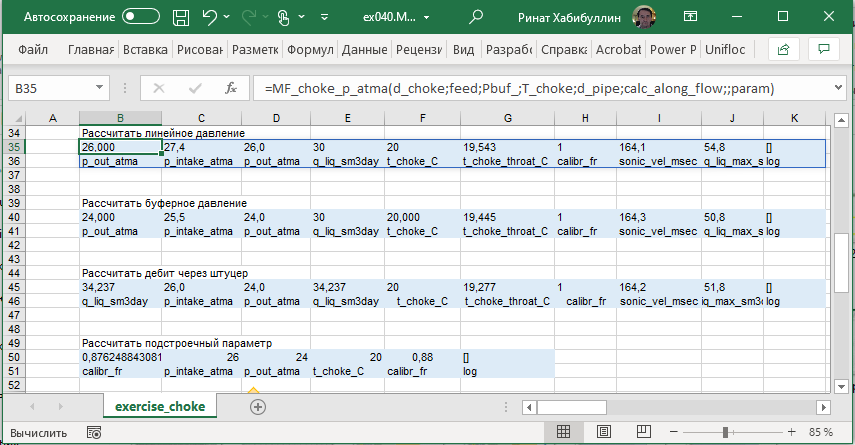
\includegraphics[width=1\linewidth]{choke_array_out}}
	\caption{Пример вывода результата расчета в массив}
	\label{ris:choke_array_out}
\end{figure}

Функции расчёта штуцера поддерживают вычисления потока чистого газа через штуцер. Для этого в PVT строке надо установить \mintinline{vb.net}{gas_only=True} и задать расход газа параметром \mintinline{vb.net}{q_gas_sm3day} в соответствующей функции. 

\subsection{MF\_choke\_p\_atma – Расчет давления на входе или на выходе штуцера}
Функция позволяет рассчитать давление на входе или выходе штуцера по известному давлению на противоположном конце при известных параметрах потока (дебите жидкости, обводнённости, газовому фактору). Расчёт проводится по корреляции Перкинса \cite{Perkins_1993} с учётом многофазного потока. 
 
\putlisting{listings/MF_choke_p_atma.lst}

Если при формировании PVT строки задать параметр \mintinline{vb.net}{gas_only=True}, то расчет будет проведен для потока газа заданного параметром \mintinline{vb.net}{q_gas_sm3day}.

%\subsection{MF\_dp\_choke\_atm – Расчёт перепада давления в штуцере}
%Функция позволяет рассчитать по известному линейному давлению и дебиту или по известному буферному давлению и дебиту перепад давления.  Расчет проводится по корреляции Перкинса \cite{Perkins_1993} с учетом многофазного потока.  
%Функция возвращает перепад давления и температуры в виде массива.
%\putlisting{listings/MF_dp_choke_atm.lst}


\subsection{MF\_choke\_q\_sm3day – функция расчёта дебита жидкости через штуцер}
Функция позволяет рассчитать по известному буферному давлению и линейному давлению дебит жидкости. Расчет  проводится по корреляции Перкинса \cite{Perkins_1993} с учетом многофазного потока.  

\putlisting{listings/MF_choke_q_sm3day.lst}

Если при формировании PVT строки задать параметр \mintinline{vb.net}{gas_only=True}, то расчет будет проведен для потока газа.

\subsection{MF\_choke\_calibr\_fast – простая и быстрая функция настройки модели штуцера}
Функция позволяет рассчитать корректирующий фактор для модели штуцера, позволяющий согласовать результаты замеров давления и дебита. Расчет проводится по корреляции Перкинса \cite{Perkins_1993} с учетом многофазного потока.  

Это быстрый способ расчета калибровочного коэффициента. По факту он просто вычисляется исходя из модели штуцера.
В более сложной функции калибровки \mintinline{vb.net}{MF_calibr_choke} расчет будет проводится дольше, так как подстроечные параметры подбираются итеративным алгоритмом, зато имеется возможность подбора нескольких различных параметров.

\putlisting{listings/MF_choke_calibr_fast.lst}

Если при формировании PVT строки задать параметр \mintinline{vb.net}{gas_only=True}, то расчет проведен не будет.


\subsection{MF\_choke\_calibr – продвинутая функция настройки модели штуцера}
Функция позволяет рассчитать корректирующий фактор для модели штуцера, позволяющий согласовать результаты замеров давления и дебита. Расчет проводится по корреляции Перкинса \cite{Perkins_1993} с учетом многофазного потока.  

Настройка может проводиться за счет подбора различных параметров. Тип калибровки выбирается параметром \mintinline{vb.net}{calibr_type} В текущей реализации может быть подобран только один из перечисленных ниже параметров.

\begin{itemize}
	\item \mintinline{vb.net}{calibr_type=0} Калибровочный коэффициент многофазной корреляции для гравитационной составляющей  $c_{calibr\_grav}$. Ищется в диапазоне от 0.5 до 1.5.
	\item \mintinline{vb.net}{calibr_type=1} Калибровочный коэффициент многофазной корреляции для трения $c_{calibr\_fric}$. Ищется в диапазоне от 0.5 до 1.5.
	\item \mintinline{vb.net}{calibr_type=2} Газовый фактор $R_p$. Ищется в диапазоне $[20, 2 R_p]$ относительно заданного газового фактора. 
	\item \mintinline{vb.net}{calibr_type=3} Обводненность $f_w$.  Значение ищется в диапазоне $[0, 1]$.  
	\item \mintinline{vb.net}{calibr_type=4} Дебит жидкости \(Q_{liq}\). Значение ищется в диапазоне от \([0, Q_{liq}*1.5]\) относительно заданного дебита жидкости. 	 
	\item \mintinline{vb.net}{calibr_type=5} Дебит жидкости \(Q_{gas}\). Значение ищется  в диапазоне от \([0, Q_{gas}*2]\) относительно заданного дебита газа или в диапазоне \([0,10000]\) м3/сут если дебит газа не задан. 	
\end{itemize}

Результат расчета - массив с подобранным параметром или сообщением о невозможности подбора, информацией о количестве итераций. 

\putlisting{listings/MF_choke_calibr.lst}

Если при формировании PVT строки задать параметр \mintinline{vb.net}{gas_only=True}, то расчет проведен не будет.

\newpage
\section{Расчет многофазного потока в трубе}

\begin{comment}
Для расчёта участка трубы с использованием пользовательских функций \unf{} применяется схема показанная на рисунке \ref{ris:Pipe_scheme_1}.

Участок трубы задаётся прямым с постоянным наклоном $\theta$  длиной $L$, постоянного диаметра $d$. Угол  $\theta$ меняется от -90 до 90 градусов Цельсия. Причем положительные наклоны угла соответствуют наклону трубы вниз, а отрицательные вверх. Изначально все расчеты отлаживались для скважин, где принято, чтобы на устье координата равна нулю и росла с глубиной. Так и осталось вплоть до текущей версии \unf{}.  Направление потока в трубе задается отдельным параметром в соответствующих функциях. Следует помнить, что не все гидравлические корреляции поддерживают расчет параметров нисходящего потока (Беггс Брилл работает, для расчета нагнетательных скважин рекомендуется применять эту корреляцию с обводненностью $f_w = 100\% $, Ансари только для потока вверх). Угол наклона $\theta = 0 $ соответствует потоку в горизонтальном участке трубопровода.

Труба имеет постоянную по всей длине шероховатость стенок. Шероховатость влияет на коэффициент трения при расчете потока и проявляется при относительно больших скоростях потока. Подробнее про шероховатость и трение в потоке жидкости можно почитать в \cite{Bratland_Pipe_Flow_1}

\begin{figure}[H]
	\begin{center}
		

\tikzset{every picture/.style={line width=0.75pt}} %set default line width to 0.75pt        

\begin{tikzpicture}[x=0.75pt,y=0.75pt,yscale=-1,xscale=1]
%uncomment if require: \path (0,395); %set diagram left start at 0, and has height of 395

%Shape: Can [id:dp21085002105230832] 
\draw  [fill={rgb, 255:red, 250; green, 245; blue, 184 }  ,fill opacity=1 ][line width=2.25]  (210.09,26.86) -- (518.1,277.18) .. controls (520.79,279.36) and (517.07,288.39) .. (509.8,297.34) .. controls (502.52,306.29) and (494.45,311.77) .. (491.76,309.59) -- (183.75,59.28) .. controls (181.07,57.09) and (184.79,48.07) .. (192.06,39.12) .. controls (199.33,30.17) and (207.41,24.68) .. (210.09,26.86) .. controls (212.78,29.05) and (209.06,38.07) .. (201.78,47.02) .. controls (194.51,55.97) and (186.44,61.46) .. (183.75,59.28) ;
%Shape: Arc [id:dp4551319717308462] 
\draw  [draw opacity=0] (246.53,26.24) .. controls (246.15,29.58) and (245.2,32.91) .. (243.64,36.1) .. controls (241.82,39.8) and (239.34,42.95) .. (236.42,45.5) -- (216.71,22.87) -- cycle ; \draw   (246.53,26.24) .. controls (246.15,29.58) and (245.2,32.91) .. (243.64,36.1) .. controls (241.82,39.8) and (239.34,42.95) .. (236.42,45.5) ;
%Straight Lines [id:da16470020046137734] 
\draw    (183.75,59.28) -- (135.67,118.67) ;
%Straight Lines [id:da017961424869073594] 
\draw    (491.76,309.59) -- (453,362) ;
%Straight Lines [id:da6308247520600512] 
\draw    (159.71,88.97) -- (472.38,335.8) ;
%Straight Lines [id:da6626067218684242] 
\draw    (339.67,156) -- (305.89,128.6) ;
\draw [shift={(304.33,127.34)}, rotate = 399.05] [color={rgb, 255:red, 0; green, 0; blue, 0 }  ][line width=0.75]    (10.93,-3.29) .. controls (6.95,-1.4) and (3.31,-0.3) .. (0,0) .. controls (3.31,0.3) and (6.95,1.4) .. (10.93,3.29)   ;
%Straight Lines [id:da9499771576021536] 
\draw    (102.33,25) -- (621,23.67) ;
%Straight Lines [id:da9922530196016488] 
\draw    (210.09,26.86) -- (624.45,362.41) ;
\draw [shift={(626,363.67)}, rotate = 219] [color={rgb, 255:red, 0; green, 0; blue, 0 }  ][line width=0.75]    (10.93,-3.29) .. controls (6.95,-1.4) and (3.31,-0.3) .. (0,0) .. controls (3.31,0.3) and (6.95,1.4) .. (10.93,3.29)   ;

% Text Node
\draw (253,39.67) node    {$\theta $};
% Text Node
\draw (299,216.33) node  [rotate=-2.44]  {$L$};
% Text Node
\draw (524.33,308.33) node  [rotate=-0.74]  {$P_{in}$};
% Text Node
\draw (165.33,38.67) node  [rotate=-0.74]  {$P_{out}$};
% Text Node
\draw (355.67,162.67) node  [rotate=-0.61]  {$Q_{liq}$};
% Text Node
\draw (210,13.33) node  [rotate=-2.44]  {$0$};
% Text Node
\draw (527,264.33) node  [rotate=-2.44]  {$L$};


\end{tikzpicture}
		\caption{Схема трубы принятая для расчётов с использованием пользовательских функций}
		\label{ris:Pipe_scheme_1}
	\end{center}
\end{figure}

Для проведения расчета в трубе вдоль нее вводится система координат. Координата соответствует измеренной длине трубы. Расчет давления проводится относительно введенных координат. 
Для расчёта распределения давления в трубе необходимо задать граничное значение давления на одном из концов трубы. Оно задается параметром  \mintinline{vb.net}{p_calc_from_atma}. Температура потока в точке, где задается давление, определяется параметром  \mintinline{vb.net}{t_calc_from_C}, температура на другом конце трубы  параметром \mintinline{vb.net}{t_calc_to_C}.  В функциях где надо задать значение давления с двух сторон, используются обозначения \mintinline{vb.net}{p_calc_from_atma} и \mintinline{vb.net}{p_calc_to_atma} соответственно обозначающие давление на разных сторонах трубы. 



\begin{figure}[H]
	\begin{minipage}[h]{0.48\linewidth}
		\centering 
		

\tikzset{every picture/.style={line width=0.5pt}} %set default line width to 0.75pt        

\begin{tikzpicture}[x=0.75pt,y=0.75pt, yscale=-0.6, xscale=0.6, every node/.style={scale=0.6}]
%uncomment if require: \path (0,436); %set diagram left start at 0, and has height of 436

%Right Arrow [id:dp9720124278067144] 
\draw  [fill={rgb, 255:red, 245; green, 166; blue, 35 }  ,fill opacity=1 ] (136.34,163.97) -- (382.9,361.29) -- (384.73,359) -- (394.62,374.41) -- (377.42,368.14) -- (379.25,365.85) -- (132.69,168.53) -- cycle ;
%Shape: Can [id:dp152680848758034] 
\draw  [fill={rgb, 255:red, 250; green, 245; blue, 184 }  ,fill opacity=1 ][line width=1.25]  (204.09,31.86) -- (512.1,282.18) .. controls (514.79,284.36) and (511.07,293.39) .. (503.8,302.34) .. controls (496.52,311.29) and (488.45,316.77) .. (485.76,314.59) -- (177.75,64.28) .. controls (175.07,62.09) and (178.79,53.07) .. (186.06,44.12) .. controls (193.33,35.17) and (201.41,29.68) .. (204.09,31.86) .. controls (206.78,34.05) and (203.06,43.07) .. (195.78,52.02) .. controls (188.51,60.97) and (180.44,66.46) .. (177.75,64.28) ;
%Shape: Arc [id:dp8055192315754607] 
\draw  [draw opacity=0] (240.53,31.24) .. controls (240.15,34.58) and (239.2,37.91) .. (237.64,41.1) .. controls (235.82,44.8) and (233.34,47.95) .. (230.42,50.5) -- (210.71,27.87) -- cycle ; \draw   (240.53,31.24) .. controls (240.15,34.58) and (239.2,37.91) .. (237.64,41.1) .. controls (235.82,44.8) and (233.34,47.95) .. (230.42,50.5) ;
%Straight Lines [id:da40478260011732936] 
\draw    (177.75,64.28) -- (129.67,123.67) ;
%Straight Lines [id:da43296084157104864] 
\draw    (485.76,314.59) -- (447,367) ;
%Straight Lines [id:da9299887303985335] 
\draw    (153.71,93.97) -- (466.38,340.8) ;
%Straight Lines [id:da6924385063009486] 
\draw    (365.67,189) -- (406.96,223.09) ;
\draw [shift={(408.5,224.36)}, rotate = 219.54] [color={rgb, 255:red, 0; green, 0; blue, 0 }  ][line width=0.75]    (10.93,-3.29) .. controls (6.95,-1.4) and (3.31,-0.3) .. (0,0) .. controls (3.31,0.3) and (6.95,1.4) .. (10.93,3.29)   ;
%Straight Lines [id:da8745382431398607] 
\draw    (96.33,30) -- (615,28.67) ;
%Straight Lines [id:da52189718709475] 
\draw    (204.09,31.86) -- (618.45,367.41) ;
\draw [shift={(620,368.67)}, rotate = 219] [color={rgb, 255:red, 0; green, 0; blue, 0 }  ][line width=0.75]    (10.93,-3.29) .. controls (6.95,-1.4) and (3.31,-0.3) .. (0,0) .. controls (3.31,0.3) and (6.95,1.4) .. (10.93,3.29)   ;

% Text Node
\draw  [color={rgb, 255:red, 0; green, 0; blue, 0 }  ,draw opacity=1 ][fill={rgb, 255:red, 245; green, 166; blue, 35 }  ,fill opacity=1 ]  (106, 146.37) circle [x radius= 29.33, y radius= 29.33]   ;
\draw (106,146.37) node  [font=\large,rotate=-359.71]  {$P_{from}$};
% Text Node
\draw  [fill={rgb, 255:red, 245; green, 166; blue, 35 }  ,fill opacity=1 ]  (423.67, 393.37) circle [x radius= 21.22, y radius= 21.22]   ;
\draw (423.67,393.37) node  [font=\large,rotate=-0.74]  {$P_{to}$};
% Text Node
\draw (247,44.67) node    {$\theta $};
% Text Node
\draw (293,221.33) node  [rotate=-2.44]  {$L$};
% Text Node
\draw (518.33,313.33) node  [rotate=-0.74]  {$P_{in}$};
% Text Node
\draw (159.33,43.67) node  [rotate=-0.74]  {$P_{out}$};
% Text Node
\draw (349.67,167.67) node  [rotate=-0.61]  {$Q_{liq}$};
% Text Node
\draw (204,18.33) node  [rotate=-2.44]  {$0$};
% Text Node
\draw (521,269.33) node  [rotate=-2.44]  {$L$};


\end{tikzpicture} \\a) \mintinline{vb.net}{calc_flow_direction=11}\\ \ 
	\end{minipage}
	\hfill
	\begin{minipage}[h]{0.48\linewidth}
		\centering
		

\tikzset{every picture/.style={line width=0.5pt}} %set default line width to 0.75pt        

\begin{tikzpicture}[x=0.75pt,y=0.75pt, yscale=-0.6, xscale=0.6, every node/.style={scale=0.6}]
%uncomment if require: \path (0,436); %set diagram left start at 0, and has height of 436

%Right Arrow [id:dp20094367581683348] 
\draw  [fill={rgb, 255:red, 245; green, 166; blue, 35 }  ,fill opacity=1 ] (136.34,163.97) -- (382.9,361.29) -- (384.73,359) -- (394.62,374.41) -- (377.42,368.14) -- (379.25,365.85) -- (132.69,168.53) -- cycle ;
%Shape: Can [id:dp40587490015631356] 
\draw  [fill={rgb, 255:red, 250; green, 245; blue, 184 }  ,fill opacity=1 ][line width=1.25]  (204.09,31.86) -- (512.1,282.18) .. controls (514.79,284.36) and (511.07,293.39) .. (503.8,302.34) .. controls (496.52,311.29) and (488.45,316.77) .. (485.76,314.59) -- (177.75,64.28) .. controls (175.07,62.09) and (178.79,53.07) .. (186.06,44.12) .. controls (193.33,35.17) and (201.41,29.68) .. (204.09,31.86) .. controls (206.78,34.05) and (203.06,43.07) .. (195.78,52.02) .. controls (188.51,60.97) and (180.44,66.46) .. (177.75,64.28) ;
%Shape: Arc [id:dp3380417833680267] 
\draw  [draw opacity=0] (240.53,31.24) .. controls (240.15,34.58) and (239.2,37.91) .. (237.64,41.1) .. controls (235.82,44.8) and (233.34,47.95) .. (230.42,50.5) -- (210.71,27.87) -- cycle ; \draw   (240.53,31.24) .. controls (240.15,34.58) and (239.2,37.91) .. (237.64,41.1) .. controls (235.82,44.8) and (233.34,47.95) .. (230.42,50.5) ;
%Straight Lines [id:da9189033332871033] 
\draw    (177.75,64.28) -- (129.67,123.67) ;
%Straight Lines [id:da9657628883300458] 
\draw    (485.76,314.59) -- (447,367) ;
%Straight Lines [id:da8924810128283758] 
\draw    (153.71,93.97) -- (466.38,340.8) ;
%Straight Lines [id:da8209365759070482] 
\draw    (333.67,161) -- (299.89,133.6) ;
\draw [shift={(298.33,132.34)}, rotate = 399.05] [color={rgb, 255:red, 0; green, 0; blue, 0 }  ][line width=0.75]    (10.93,-3.29) .. controls (6.95,-1.4) and (3.31,-0.3) .. (0,0) .. controls (3.31,0.3) and (6.95,1.4) .. (10.93,3.29)   ;
%Straight Lines [id:da6797754281808239] 
\draw    (96.33,30) -- (615,28.67) ;
%Straight Lines [id:da5030952677621108] 
\draw    (204.09,31.86) -- (618.45,367.41) ;
\draw [shift={(620,368.67)}, rotate = 219] [color={rgb, 255:red, 0; green, 0; blue, 0 }  ][line width=0.75]    (10.93,-3.29) .. controls (6.95,-1.4) and (3.31,-0.3) .. (0,0) .. controls (3.31,0.3) and (6.95,1.4) .. (10.93,3.29)   ;

% Text Node
\draw  [color={rgb, 255:red, 0; green, 0; blue, 0 }  ,draw opacity=1 ][fill={rgb, 255:red, 245; green, 166; blue, 35 }  ,fill opacity=1 ]  (106, 146.37) circle [x radius= 29.33, y radius= 29.33]   ;
\draw (106,146.37) node  [font=\large,rotate=-359.71]  {$P_{from}$};
% Text Node
\draw  [fill={rgb, 255:red, 245; green, 166; blue, 35 }  ,fill opacity=1 ]  (423.67, 393.37) circle [x radius= 21.22, y radius= 21.22]   ;
\draw (423.67,393.37) node  [font=\large,rotate=-0.74]  {$P_{to}$};
% Text Node
\draw (247,44.67) node    {$\theta $};
% Text Node
\draw (293,221.33) node  [rotate=-2.44]  {$L$};
% Text Node
\draw (518.33,313.33) node  [rotate=-0.74]  {$P_{in}$};
% Text Node
\draw (159.33,43.67) node  [rotate=-0.74]  {$P_{out}$};
% Text Node
\draw (349.67,167.67) node  [rotate=-0.61]  {$Q_{liq}$};
% Text Node
\draw (204,18.33) node  [rotate=-2.44]  {$0$};
% Text Node
\draw (521,269.33) node  [rotate=-2.44]  {$L$};


\end{tikzpicture} \\b) \mintinline{vb.net}{calc_flow_direction=10}\\ \ 
	\end{minipage}
	\vfill
	\begin{minipage}[h]{0.48\linewidth}
		\centering 
		

\tikzset{every picture/.style={line width=0.5pt}} %set default line width to 0.75pt        

\begin{tikzpicture}[x=0.75pt,y=0.75pt, yscale=-0.55, xscale=0.55, every node/.style={scale=0.55}]
%uncomment if require: \path (0,436); %set diagram left start at 0, and has height of 436

%Right Arrow [id:dp614954492412991] 
\draw  [fill={rgb, 255:red, 245; green, 166; blue, 35 }  ,fill opacity=1 ] (393.73,367.97) -- (149.14,168.2) -- (147.29,170.47) -- (137.56,154.96) -- (154.7,161.41) -- (152.84,163.67) -- (397.43,363.44) -- cycle ;
%Shape: Can [id:dp5051217098754548] 
\draw  [fill={rgb, 255:red, 250; green, 245; blue, 184 }  ,fill opacity=1 ][line width=1.25]  (204.09,31.86) -- (512.1,282.18) .. controls (514.79,284.36) and (511.07,293.39) .. (503.8,302.34) .. controls (496.52,311.29) and (488.45,316.77) .. (485.76,314.59) -- (177.75,64.28) .. controls (175.07,62.09) and (178.79,53.07) .. (186.06,44.12) .. controls (193.33,35.17) and (201.41,29.68) .. (204.09,31.86) .. controls (206.78,34.05) and (203.06,43.07) .. (195.78,52.02) .. controls (188.51,60.97) and (180.44,66.46) .. (177.75,64.28) ;
%Shape: Arc [id:dp25764672357613594] 
\draw  [draw opacity=0] (240.53,31.24) .. controls (240.15,34.58) and (239.2,37.91) .. (237.64,41.1) .. controls (235.82,44.8) and (233.34,47.95) .. (230.42,50.5) -- (210.71,27.87) -- cycle ; \draw   (240.53,31.24) .. controls (240.15,34.58) and (239.2,37.91) .. (237.64,41.1) .. controls (235.82,44.8) and (233.34,47.95) .. (230.42,50.5) ;
%Straight Lines [id:da21971571097244458] 
\draw    (177.75,64.28) -- (129.67,123.67) ;
%Straight Lines [id:da9225249988390838] 
\draw    (485.76,314.59) -- (447,367) ;
%Straight Lines [id:da5713805287673805] 
\draw    (153.71,93.97) -- (466.38,340.8) ;
%Straight Lines [id:da19512561690606955] 
\draw    (363.67,187) -- (402.46,218.92) ;
\draw [shift={(404,220.19)}, rotate = 219.45] [color={rgb, 255:red, 0; green, 0; blue, 0 }  ][line width=0.75]    (10.93,-3.29) .. controls (6.95,-1.4) and (3.31,-0.3) .. (0,0) .. controls (3.31,0.3) and (6.95,1.4) .. (10.93,3.29)   ;
%Straight Lines [id:da9534565618447843] 
\draw    (96.33,30) -- (615,28.67) ;
%Straight Lines [id:da4946421064792441] 
\draw    (204.09,31.86) -- (618.45,367.41) ;
\draw [shift={(620,368.67)}, rotate = 219] [color={rgb, 255:red, 0; green, 0; blue, 0 }  ][line width=0.75]    (10.93,-3.29) .. controls (6.95,-1.4) and (3.31,-0.3) .. (0,0) .. controls (3.31,0.3) and (6.95,1.4) .. (10.93,3.29)   ;

% Text Node
\draw  [color={rgb, 255:red, 0; green, 0; blue, 0 }  ,draw opacity=1 ][fill={rgb, 255:red, 245; green, 166; blue, 35 }  ,fill opacity=1 ]  (425, 392.37) circle [x radius= 29.33, y radius= 29.33]   ;
\draw (425,392.37) node  [font=\large,rotate=-359.71]  {$P_{from}$};
% Text Node
\draw  [fill={rgb, 255:red, 245; green, 166; blue, 35 }  ,fill opacity=1 ]  (115.67, 138.37) circle [x radius= 21.22, y radius= 21.22]   ;
\draw (115.67,138.37) node  [font=\large,rotate=-0.74]  {$P_{to}$};
% Text Node
\draw (247,44.67) node    {$\theta $};
% Text Node
\draw (293,221.33) node  [rotate=-2.44]  {$L$};
% Text Node
\draw (518.33,313.33) node  [rotate=-0.74]  {$P_{in}$};
% Text Node
\draw (159.33,43.67) node  [rotate=-0.74]  {$P_{out}$};
% Text Node
\draw (349.67,167.67) node  [rotate=-0.61]  {$Q_{liq}$};
% Text Node
\draw (204,18.33) node  [rotate=-2.44]  {$0$};
% Text Node
\draw (521,269.33) node  [rotate=-2.44]  {$L$};


\end{tikzpicture} \\c) \mintinline{vb.net}{calc_flow_direction=01}\\ \ 
	\end{minipage}
	\hfill
	\begin{minipage}[h]{0.48\linewidth}
		\centering 
			
	\tikzset{every picture/.style={line width=0.75pt}} %set default line width to 0.75pt        
	
	\begin{tikzpicture}[x=0.75pt,y=0.75pt,yscale=-1,xscale=1]
	%uncomment if require: \path (0,453); %set diagram left start at 0, and has height of 453
	
	%Shape: Can [id:dp7385102204739014] 
	\draw  [fill={rgb, 255:red, 250; green, 245; blue, 184 }  ,fill opacity=1 ][line width=2.25]  (198.23,370.28) -- (505.15,118.62) .. controls (507.82,116.43) and (515.92,121.88) .. (523.23,130.8) .. controls (530.54,139.72) and (534.3,148.72) .. (531.63,150.92) -- (224.71,402.57)(198.23,370.28) .. controls (200.9,368.08) and (209,373.54) .. (216.31,382.45) .. controls (223.63,391.37) and (227.39,400.38) .. (224.71,402.57) .. controls (222.03,404.77) and (213.94,399.32) .. (206.62,390.4) .. controls (199.31,381.48) and (195.55,372.47) .. (198.23,370.28) -- cycle ;
	%Shape: Arc [id:dp4602786709186524] 
	\draw  [draw opacity=0] (247.54,383.1) .. controls (249.72,385.66) and (251.51,388.62) .. (252.76,391.95) .. controls (254.22,395.8) and (254.84,399.77) .. (254.7,403.64) -- (224.71,402.57) -- cycle ; \draw   (247.54,383.1) .. controls (249.72,385.66) and (251.51,388.62) .. (252.76,391.95) .. controls (254.22,395.8) and (254.84,399.77) .. (254.7,403.64) ;
	%Straight Lines [id:da5353213855148988] 
	\draw    (145.83,313.7) -- (198.23,370.28) ;
	
	
	%Straight Lines [id:da6371642797081225] 
	\draw    (460.06,65.51) -- (505.15,118.62) ;
	
	
	%Straight Lines [id:da5708425902799406] 
	\draw    (172.03,341.99) -- (482.6,92.07) ;
	
	
	%Straight Lines [id:da5694938455522887] 
	\draw    (377.67,250.37) -- (407,226.74) ;
	\draw [shift={(408.56,225.48)}, rotate = 501.14] [color={rgb, 255:red, 0; green, 0; blue, 0 }  ][line width=0.75]    (10.93,-3.29) .. controls (6.95,-1.4) and (3.31,-0.3) .. (0,0) .. controls (3.31,0.3) and (6.95,1.4) .. (10.93,3.29)   ;
	
	%Straight Lines [id:da47656732513988986] 
	\draw    (123,403.37) -- (603.56,403.37) ;
	\draw [shift={(605.56,403.37)}, rotate = 180] [color={rgb, 255:red, 0; green, 0; blue, 0 }  ][line width=0.75]    (10.93,-3.29) .. controls (6.95,-1.4) and (3.31,-0.3) .. (0,0) .. controls (3.31,0.3) and (6.95,1.4) .. (10.93,3.29)   ;
	
	%Right Arrow [id:dp49730840239995544] 
	\draw  [fill={rgb, 255:red, 245; green, 166; blue, 35 }  ,fill opacity=1 ] (419.38,64.16) -- (174.9,264.05) -- (176.75,266.31) -- (159.61,272.77) -- (169.34,257.26) -- (171.19,259.52) -- (415.67,59.63) -- cycle ;
	
	% Text Node
	\draw (267.67,388.7) node   {$\theta $};
	% Text Node
	\draw (303.67,212.04) node [rotate=-2.44]  {$L$};
	% Text Node
	\draw (229.33,374.04) node [rotate=-0.74]  {$P_{in}$};
	% Text Node
	\draw (509.67,137.37) node [rotate=-0.74]  {$P_{out}$};
	% Text Node
	\draw (369.67,255.04) node [rotate=-0.61]  {$Q_{liq}$};
	% Text Node
	\draw  [color={rgb, 255:red, 0; green, 0; blue, 0 }  ,draw opacity=1 ][fill={rgb, 255:red, 245; green, 166; blue, 35 }  ,fill opacity=1 ]  (444, 43.37) circle [x radius= 25.3, y radius= 25.3]   ;
	\draw (444,43.37) node [scale=1.2,rotate=-359.71]  {$P_{calc}$};
	% Text Node
	\draw  [fill={rgb, 255:red, 245; green, 166; blue, 35 }  ,fill opacity=1 ]  (129.67, 288.37) circle [x radius= 21.57, y radius= 21.57]   ;
	\draw (129.67,288.37) node [scale=1.2,rotate=-0.74]  {$P_{in}$};
	
	
	\end{tikzpicture} \\d) \mintinline{vb.net}{calc_flow_direction=00}\\ \ 
	\end{minipage}
	\caption{Схема расчёта распределения давления против потока}
	\label{ris:Pipe_scheme_1_4}
\end{figure}


Направление расчета, как и направление потока относительно введенной системы координат определяется параметром  \mintinline{vb.net}{calc_flow_direction} 

Возможны следующие варианты задания параметра расчета, смотри рисунок \ref{ris:Pipe_scheme_1_4}.
\begin{enumerate}
	\item  \mintinline{vb.net}{calc_flow_direction=11} расчет идет в направлении роста координаты, и поток идет в том же направлении, смотри рисунок \ref{ris:Pipe_scheme_1_4} a).
	
	\item  \mintinline{vb.net}{calc_flow_direction=10} расчет идет в направлении роста координаты, а поток идет в противоположном направлении, смотри рисунок \ref{ris:Pipe_scheme_1_4} b).
	
	\item  \mintinline{vb.net}{calc_flow_direction=01} расчет идет в направлении убывания координаты, а поток идет в направлении роста координаты, смотри рисунок \ref{ris:Pipe_scheme_1_4} c).
	
	\item  \mintinline{vb.net}{calc_flow_direction=00} расчет идет в направлении убывания координаты и поток идет в том же направлении, смотри рисунок \ref{ris:Pipe_scheme_1_4} d).
\end{enumerate}

Схема расчета \mintinline{vb.net}{calc_flow_direction=00} для случая вертикальной добывающей скважины соответствует расчету распределения давления "снизу вверх" - от забойного давления к устьевому, если считать что координата направлена "сверху вниз". То есть если на устье начало координат, а на забое координата равна измеренной глубине, то давление \mintinline{vb.net}{p_calc_from_atma} соответствует забойному, а \mintinline{vb.net}{p_calc_to_atma} устьевому. 


Схема расчета \mintinline{vb.net}{calc_flow_direction=11} для случая вертикальной нагнетательной скважины соответствует расчету распределения давления "сверху вниз" - от устьевого давления к забойному, если считать что координата направлена "сверху вниз". То есть если на устье начало координат, а на забое координата равна измеренной глубине, то давление \mintinline{vb.net}{p_calc_from_atma} соответствует устьевому, а \mintinline{vb.net}{p_calc_to_atma} забойному. 

\end{comment}

%\subsection{MF\_dp\_pipe\_atm – расчёт перепада давления в трубе}

%Функция позволяет рассчитать перепад давления в участке трубопровода. 
%Функция возвращает давление и температуру в виде массива.

%\putlisting{listings/MF_dp_pipe_atm.lst}

Расчет распределения давления в трубе основан на многофазных корреляциях. Выбор типа корреляции определяется параметром  \mintinline{vb.net}{hydr_corr}. В текущей версии \unf{} реализован следующий набор гидравлических корреляций:
\begin{enumerate}
	\item \mintinline{vb.net}{hydr_corr = 0}. Корреляция Беггса Брилла.
	\item \mintinline{vb.net}{hydr_corr = 1}. Корреляция Ансари.
	\item \mintinline{vb.net}{hydr_corr = 2}. Корреляция TUFFP Unified.
	\item \mintinline{vb.net}{hydr_corr = 3}. Корреляция Грея, модифицированная.
	\item \mintinline{vb.net}{hydr_corr = 4}. Корреляция Хайгедорна Брауна.
	\item \mintinline{vb.net}{hydr_corr = 5}. Корреляция Сахарова Мохова.
	\item \mintinline{vb.net}{hydr_corr = 10}. Расчет на основе плотности газа, без учета жидкости.
	
\end{enumerate}

Ниже на рисунке \ref{ris:VLP_curves} приведены результаты расчёта кривой оттока (перепада давления в вертикальной трубе) для различных корреляций, реализованных в \unf{}.

\begin{figure}[H]
	\begin{center}
	\newcommand{\dPipeDataFile}{data/dPipe.txt}
		\begin{tikzpicture}[scale=1]
		\begin{axis}[
					width=14cm,
					height=10cm,
					xlabel=$Q\; m^3 / day$,
					ylabel=$P_{wf} \; atma$,
					legend pos=south east,
					title=Pipe Pressure Drop]
		\addplot table [y=P_0, x=Q]{\dPipeDataFile};
		\addlegendentry{Beggs Brill}
		\addplot table [y=P_1, x=Q]{\dPipeDataFile};
		\addlegendentry{Ansari}
		\addplot table [y=P_2, x=Q]{\dPipeDataFile};
		\addlegendentry{Unified}
		\addplot table [y=P_3, x=Q]{\dPipeDataFile};
		\addlegendentry{Gray}
		\addplot table [y=P_4, x=Q]{\dPipeDataFile};
		\addlegendentry{Hagedorn Brown}
		\addplot table [y=P_5, x=Q]{\dPipeDataFile};
		\addlegendentry{Sakharov Mokhov}
		\end{axis}
		\end{tikzpicture}	
	\caption{Кривые характеристики многофазного потока для вертикальных труб рассчитанные с использованием различных корреляций }
	\label{ris:VLP_curves}
	\end{center}
\end{figure}

\subsection{MF\_pipe\_p\_atma – функция расчета давления на конце трубы}  

\begin{comment}
Функция позволяет рассчитать перепад давления в участке трубопровода. Функция обеспечивает несколько режимов расчёта. Некоторые особенности работы функции \mintinline{vb.net}{MF_p_pipe_atma()}
\begin{itemize}
	\item Свойства флюида в трубе определяются параметром \mintinline{vb.net}{str_PVT}, который в свою очередь может быть задан функцией \mintinline{vb.net}{PVT_encode()}.
	\item Дополнительно в поток может быть включен свободный газ. Задается параметром \mintinline{vb.net}{q_gas_sm3day} определяющим объемный расход приведенный к стандартным условиям. Свободный газ суммируется с газом определяемым исходя из заданных свойств флюида. 
	\item Если при определении \mintinline{vb.net}{str_PVT} указан параметр \mintinline{vb.net}{gas_only = 1}, то расчет распределения давления в трубе будет проводиться для газа, наличие жидкости в потоке учитываться не будет. В текущей версии \unf{} при расчете потока газа трение газа не учитывается, перепад давления в газовой линии не зависит от расхода газа, зависит только от плотности газа.
	\item Если параметр дебита жидкости  \mintinline{vb.net}{qliq_sm3day = 0}  равен нулю, расчет проводится для режима барботажа (ZNLF - zero net liquid flow) - движения газа через неподвижный столб жидкости. Расход газа должен быть задан параметром \mintinline{vb.net}{q_gas_sm3day}. В текущей версии \unf{} расчет барботажа проводится проводится за счет переключения на механистическую корреляцию Ансари. Попытка построить график зависимости перепад давления от дебита для других корреляций может дать нелогичный результат около нулевого дебита (скачек перепада давления). Рекомендуется без необходимости для \mintinline{vb.net}{qliq_sm3day = 0} не считать при построении графиков.
	\item Распределение температуры для функции расчета участка скважины ограничено одной моделью - линейного распределения температуры потока вдоль трубы. Для учета температуры необходимо задать параметры \mintinline{vb.net}{t_calc_from_C} и \mintinline{vb.net}{t_calc_to_C} определяющие температуру на концах трубы. В трубе значения будут проинтерполированы по длине. Если второй параметр 
\end{itemize}
 

Результатом работы функций является массив значений содержащий давление и температуру флюида на входе в трубу $P_{in}, T_{in}$, давление и температуру флюида на выходе из трубы $P_{out}, T_{out}$,  калибровочные коэффициент многофазной корреляции для гравитационной составляющей и для трения$c_{calibr\_grav},c_{calibr\_fric}$.  Выходной массив содержит две строки - в первой находятся значения, во второй подписи. Это позволяет при необходимости вывести только значения в той же строке в которой проводился расчет. Значение в первой строке и в первом столбце зависит от настройки функции (параметра \mintinline{vb.net}{calc_along_flow} для функции \mintinline{vb.net}{MF_p_pipe_atma}) и содержит основной результат расчета. Значения в последующих столбцах не зависят от настройки функции и показывают все результаты расчета.
Для вывода массива в Excel следует выбрать необходимый диапазон ячеек, в который будут выводится результаты в виде массива, затем ввести в адресную строку вызов функции и нажать комбинацию клавиш - Cntrl-Shift-Enter. После этого название функции в адресной строке должно отображаться в фигурных скобках, аналогично функции расчета давления в штуцере, рисунок \ref{ris:choke_array_out}. При необходимости внести коррективы в вызов функции также необходимо подтверждать свои действия комбинацией клавиш Cntrl-Shift-Enter.
\end{comment}
\putlisting{listings/MF_pipe_p_atma.lst}
\begin{comment}
Результатом работы функции является массив, содержащий давления и температуру на концах трубы, калибровочные параметры, а также значения ряда параметров между концами трубы. Вывод значений между концами трубы может быть отключен установкой \mintinline{vb.net}{out_curves=False}. При необходимости проведения массовых расчетов можно вывести только одно значение (или одну строку значений) штатными средствами Excel. 

\begin{figure}[ht]
	\center{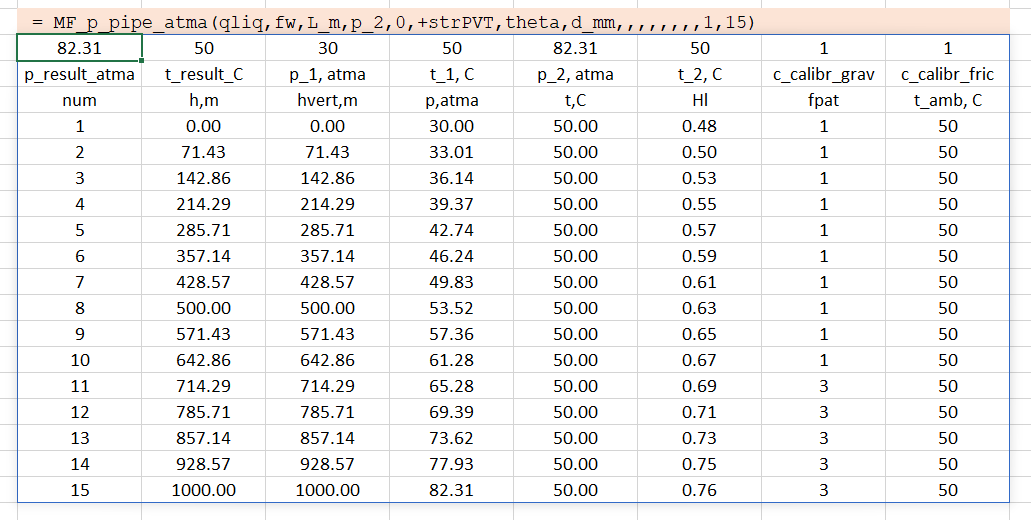
\includegraphics[width=1\linewidth]{pipe_out_example}}
	\caption{Пример вывода результатов расчета функции \mintinline{vb.net}{MF_p_pipe_atma()} для  \mintinline{vb.net}{out_curves=True} }
	\label{ris:pipe_out_example}
\end{figure}

\begin{figure}[ht]
	\center{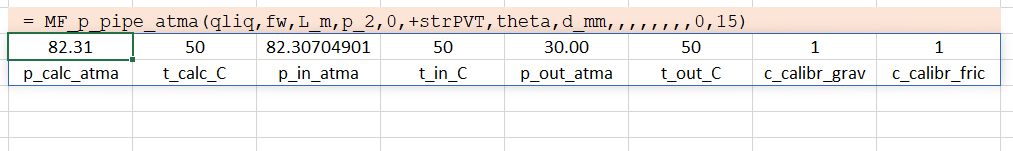
\includegraphics[width=1\linewidth]{pipe_out_example_short}}
	\caption{Пример вывода результатов расчета функции \mintinline{vb.net}{MF_p_pipe_atma()} для  \mintinline{vb.net}{out_curves=False} }
	\label{ris:pipe_out_example_short}
\end{figure}

\subsection{MF\_calibr\_pipe, MF\_calibr\_pipeline - функция калибровки расчета участка трубы}

Функция калибровки позволяет настроить модель потока в трубе под замеры давления на концах трубы. Настройка может проводиться за счет подбора различных параметров. Тип калибровки выбирается параметром \mintinline{vb.net}{calibr_type} В текущей реализации может быть подобран только один из перечисленных ниже параметров.

\begin{itemize}
	\item \mintinline{vb.net}{calibr_type=0} Калибровочный коэффициент многофазной корреляции для гравитационной составляющей  $c_{calibr\_grav}$. Ищется в диапазоне от 0.5 до 1.5.
	\item \mintinline{vb.net}{calibr_type=1} Калибровочный коэффициент многофазной корреляции для трения $c_{calibr\_fric}$. Ищется в диапазоне от 0.5 до 1.5.
	\item \mintinline{vb.net}{calibr_type=2} Газовый фактор $R_p$. Ищется в диапазоне $[20, 2 R_p]$ относительно заданного газового фактора. 
	\item \mintinline{vb.net}{calibr_type=3} Обводненность $f_w$.  Ищется в диапазоне $[0, 1]$.  
	\item \mintinline{vb.net}{calibr_type=4} Дебит жидкости \(Q_{liq} \). Ищется в диапазоне от \([0,Q_{liq}*1.5 ]\) относительно заданного дебита жидкости. 	 
	\item \mintinline{vb.net}{calibr_type=5} Дебит жидкости \(Q_{gas} \). Ищется в диапазоне от \([0,Q_{gas}*2 ]\) относительно заданного дебита газа или в диапазоне \([0,10000 ]\) м3/сут если дебит газа не задан. 	
\end{itemize}

Результат расчета - массив с подобранным параметром или сообщением о невозможности подбора, информацией о количестве итераций. 

\putlisting{listings/MF_calibr_pipe.lst}

Подбор параметра может быть осуществлен для трубопровода, в котором может быть учтен профиль и более сложная температурная модель.

\putlisting{listings/MF_calibr_pipeline.lst}



\subsection{MF\_dpdl\_atmm – функция расчета градиента давления по многофазной корреляции Ансари}  
Иногда бывает удобно/интересно посмотреть детально на результаты расчета по многофазной корреляции. Для этого можно воспользоваться данной функцией. Внимательно смотрите описание и саму функцию. Выводит ряд параметров в массиве.
\putlisting{listings/MF_dpdl_atmm.lst}

\subsection{MF\_p\_pipeline\_atma - функция расчета трубопровода с учетом профиля и температуры}

Функция расчета трубопровода \mintinline{vb.net}{MF_p_pipeline_atma()} аналогична по функциональности функции расчета сегмента трубы \mintinline{vb.net}{MF_p_pipe_atma()} за исключением следующих моментов: в трубопроводе имеется возможность учета профиля трубопровода (инклинометрии для труб в скважине), возможность учета изменения диаметров для различных участков трубопровода и возможность более детального расчета распределения температуры флюида вдоль трубопровода (скважины) для некоторых конфигураций. Также для трубопровода всегда выводятся значения параметров потока между концами трубопровода в выходном массиве, в то время для трубы такой вывод можно подавить.

Функция отличается достаточно сложным поведением из-за возможности задания параметров в различных форматах. Данное описание не претендует на полноту. Рекомендуется изучать поведение функции на примерах. Тем не менее некоторые особенности параметров функции описаны ниже.

\begin{itemize}
	\item Параметр 	\mintinline{vb.net}{h_list_m} определяет траекторию скважины или трубопровода. Если задано одно число (или ссылка на ячейку с числом) то оно определяет длину трубопровода. Если задан двумерный массив (или ссылка на range) содержащий измеренные и вертикальные глубины, то задается траектория трубы/скважины. 
	\item Параметр 	\mintinline{vb.net}{diam_list_mm} определяет внутренний диаметр скважины или трубопровода. Если задано одно число (или ссылка на ячейку с числом) то оно определяет единый диаметр для всего трубопровода. Если задан двумерный массив (или ссылка на range) содержащий измеренные глубины и значения диаметров, то задается составной трубопровод с участками разных диаметров. 
	\item Параметр \mintinline{vb.net}{t_val} задает распределение температуры в трубопроводе или в пространстве окружающем трубопровод или скважину. Предполагается, что распределение температуры зависит от вертикальной глубины (модель больше рассчитана на скважину). Задается в виде двумерного массива (или объекта range) вертикальных глубин и температур. Если задано одно число - то модель расчета температуры будет линейная вдоль измеренной длины, а само число определяет температуру на втором конце трубы. Если задан двумерный массив значений, то модель расчета температуры определяется параметром \mintinline{vb.net}{temp_method}
	\item Параметр \mintinline{vb.net}{temp_method} определяет метод расчета распределения температуры. Для \mintinline{vb.net}{temp_method=2} используется метод с учетом эмиссии тепла в окружающее пространство. В текущей версии \unf{} для этого метода регулировка параметров теплопередачи возможна только в коде VBA. Для корректировки необходимо задать параметры объекта класса  \mintinline{vb.net}{CAmbientFormation}. Для примера смотри конструктор класса  \mintinline{vb.net}{CAmbientFormation.Class_Initialize}
	
\end{itemize}


\putlisting{listings/MF_p_pipeline_atma.lst}

Результатом работы функции является массив, содержащий давления и температуру на концах трубы, калибровочные параметры, а также значения ряда параметров между концами трубопровода.

\begin{figure}[ht]
	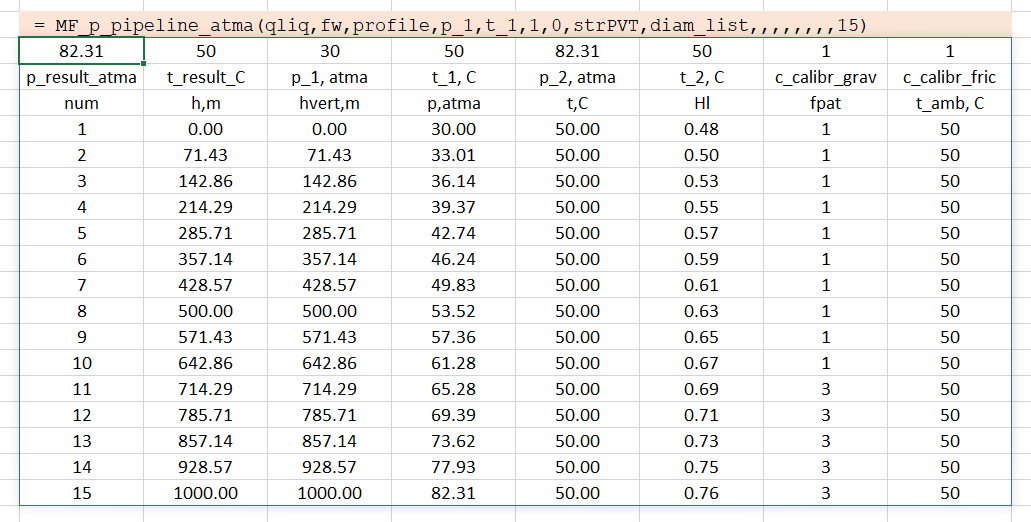
\includegraphics[width=1\linewidth]{pipeline_out_example}
	\caption{Пример вывода результатов расчета функции \mintinline{vb.net}{MF_p_pipeline_atma()}}
	\label{ris:pipeline_out_example}
\end{figure}
\end{comment}

\newpage

